% PAKETE UND DOKUMENTKONFIGURATION
\documentclass[10pt, a4paper]{article}

% Encoding für Umlaute
\usepackage[utf8]{inputenc}
\usepackage[T1]{fontenc}

% Silbentrennung
\usepackage[ngerman]{babel}

% erweiterte Matheumgebungen
\usepackage{amsmath}

% zusätzliche mathematische Schriftarten
\usepackage{amsfonts}

% verschiedene mathematische Symbole
\usepackage{amssymb}

% Einheiten setzen z.B. \SI{10}{\kilo\gram\meter\per\second\squared}
% Fehler: \SI{10 +- 0,2e-4}{\metre}
\usepackage{siunitx}
\sisetup{
  output-decimal-marker={,},
  separate-uncertainty
}

% Randbreiten
\usepackage[left=3.5cm,right=3.5cm,top=3cm,bottom=3cm,twoside]{geometry}

% Bilder einfügen
\usepackage{graphicx}

% Verweise innerhalb des Dokuments
\usepackage{hyperref}
\hypersetup{
	colorlinks = true,
	allcolors = {black}
}

% bessere Tabellenlayouts
\usepackage{booktabs}

% Tiefe des Inhaltsverzeichnisses (Level: 1 sections, 2 subsections,
% 3 subsubsections)
\setcounter{tocdepth}{2}

% manuelle Angabe zur Silbentrennung (mehrere Wörter mit Leerzeichen in {} schreiben)
\hyphenation{Rönt-gen-strah-lung}

% DOKUMENTINFORMATIONEN
\title{P428 \\ Röntgenstrahlung und Materialanalyse}

\author{Christopher Deutsch\footnote{christopher.deutsch@uni-bonn.de} \and Christian Bespin\footnote{christian.bespin@uni-bonn.de}}

\date{\today}

\begin{document}

\maketitle

% DURCHFÜHRUNGSDATUM UND ASSISTENT
\begin{center}
\begin{tabular}{l r}
Durchführung: & 3./4. November 2014 \\
Gruppe: & $\alpha$ 2 \\
Assistent: & Peter Klassen
\end{tabular}
\end{center}

% ZUSAMMENFASSUNG
\begin{abstract}
\noindent
% Text
\end{abstract}

% INHALTSVERZEICHNIS
\tableofcontents
% Neue Seite nach TOC
\newpage

% INHALT VERSUCHSPROTOKOLL

\section{Grundlagen}
\subsection{Röntgenstrahlung}
Als Röntgenstrahlung wird der Teil des elektromagnetischen Spektrums mit Photon-Energien zwischen \SI{100}{\electronvolt} und \SI{100}{\kilo\electronvolt} bezeichnet, wobei diese Grenzen nicht scharf sind und deshalb oft hinsichtlich der Strahlungsquelle eine Einordnung vollzogen wird.

\subsubsection{Erzeugung}
Es gibt zwei typische Erzeugungsmethoden von Röntgenstrahlung, welche auf dem Beschuss eines \emph{Targets} mit einem hochenergetischen Elektronenstrahl bestehen.
Die beiden Strahlungsarten, welche in der Praxis oft zusammen auftreten sind:
\begin{itemize}
  \item \textbf{Bremsstrahlung:} Die bei der Streuung der geladenen Elektronen an den Kernen des Targets vollzogene Geschwindigkeitsänderung des Elektrons, führt zur Emission eines Photons.
  Das so entstandene Spektrum ist kontinuierlich, wobei die maximale Photonenenergie gegeben ist durch die kinetische Energie der einfallenden Elektronen, welche durch deren Beschleunigungsspannung $U$ gegeben ist.
  Überträgt das Elektron seine gesamte Energie auf ein einzelnes Photon:
  \begin{align}
    &E_\mathrm{kin. e^-} = h \cdot \nu_\mathrm{max} = \frac{hc}{\lambda_\mathrm{min}}
  \end{align}
  so ist diese Grenze gegeben durch das \textbf{Duane-Hunt-Gesetz}
  \begin{align}
    \lambda_\mathrm{min} = \frac{h c}{e U} \quad \text{(Duane-Hunt-Gesetz)}
  \end{align}
  (BILD VON SPEKTRALVERTEILUNG und evtl. Kramers-Gesetz)

  Eine Quelle für reine Bremsstrahlung sind Synchrotronstrahlungsquellen.

  \item \textbf{charakteristische Strahlung:} Die einfallende hochenergetische Elektronenstrahlung ionisiert ein Elektron der inneren Schale eines Targetatoms.
  Dadurch entsteht ein freier Zustand, welcher durch ein Elektron einer weiter äußeren Schale eingenommen werden kann.
  Durch den Übergang wird ein Photon emittiert, dessen Energie gleich der Energiedifferenz der beiden Zustände ist.
  Aufgrund dieser Abhängigkeit von der elektronisches Struktur des Targetatoms, ist das emittierte, diskrete Spektrum charakteristisch für das verwendete (Target)-Material.
  Außerdem weist das emittierte Spektrum die Aufspaltung der Energieniveaus aufgrund von Fein- und Hyperfeinstruktur auf.
  (BILD VON SPEKTRALVERTEILUNG)
\end{itemize}
In der Praxis treten beide Effekte bei der Erzeugung von Röntgenstrahlen in sogennanten Röntgenröhren auf.

Eine \textbf{Röntgenröhre} besteht aus einem evakuierten Glaskolben mit einer Anordnung von geheizter Kathode und Anode aus Targetmaterial.
Zwischen Kathode und Anode wird die Beschleunigungsspannung $U$ angelegt, sodass beim Heizen der Kathode mit der Heizspannung $U_\mathrm{Heiz}$ aufgrund des glühelektrischen Effekts ein Teil der Elektronen die Austrittsarbeit der Kathode überwinden kann und durch die Beschleunigungsspannung $U$ in Richtung der Anode beschleunigt werden.
Nachdem die Beschleunigungsspannung $U$ durchlaufen wurde, treffen die Elektronen mit der Energie $e U$ auf das Anodenmaterial und erzeugen dabei Bremsstrahlung sowie charakteristische Strahlung, welche durch ein für Röntgenstrahlung durchlässiges Fenster im Glaskolben aus der Röhre austreten können.
\begin{figure}[h]
\centering
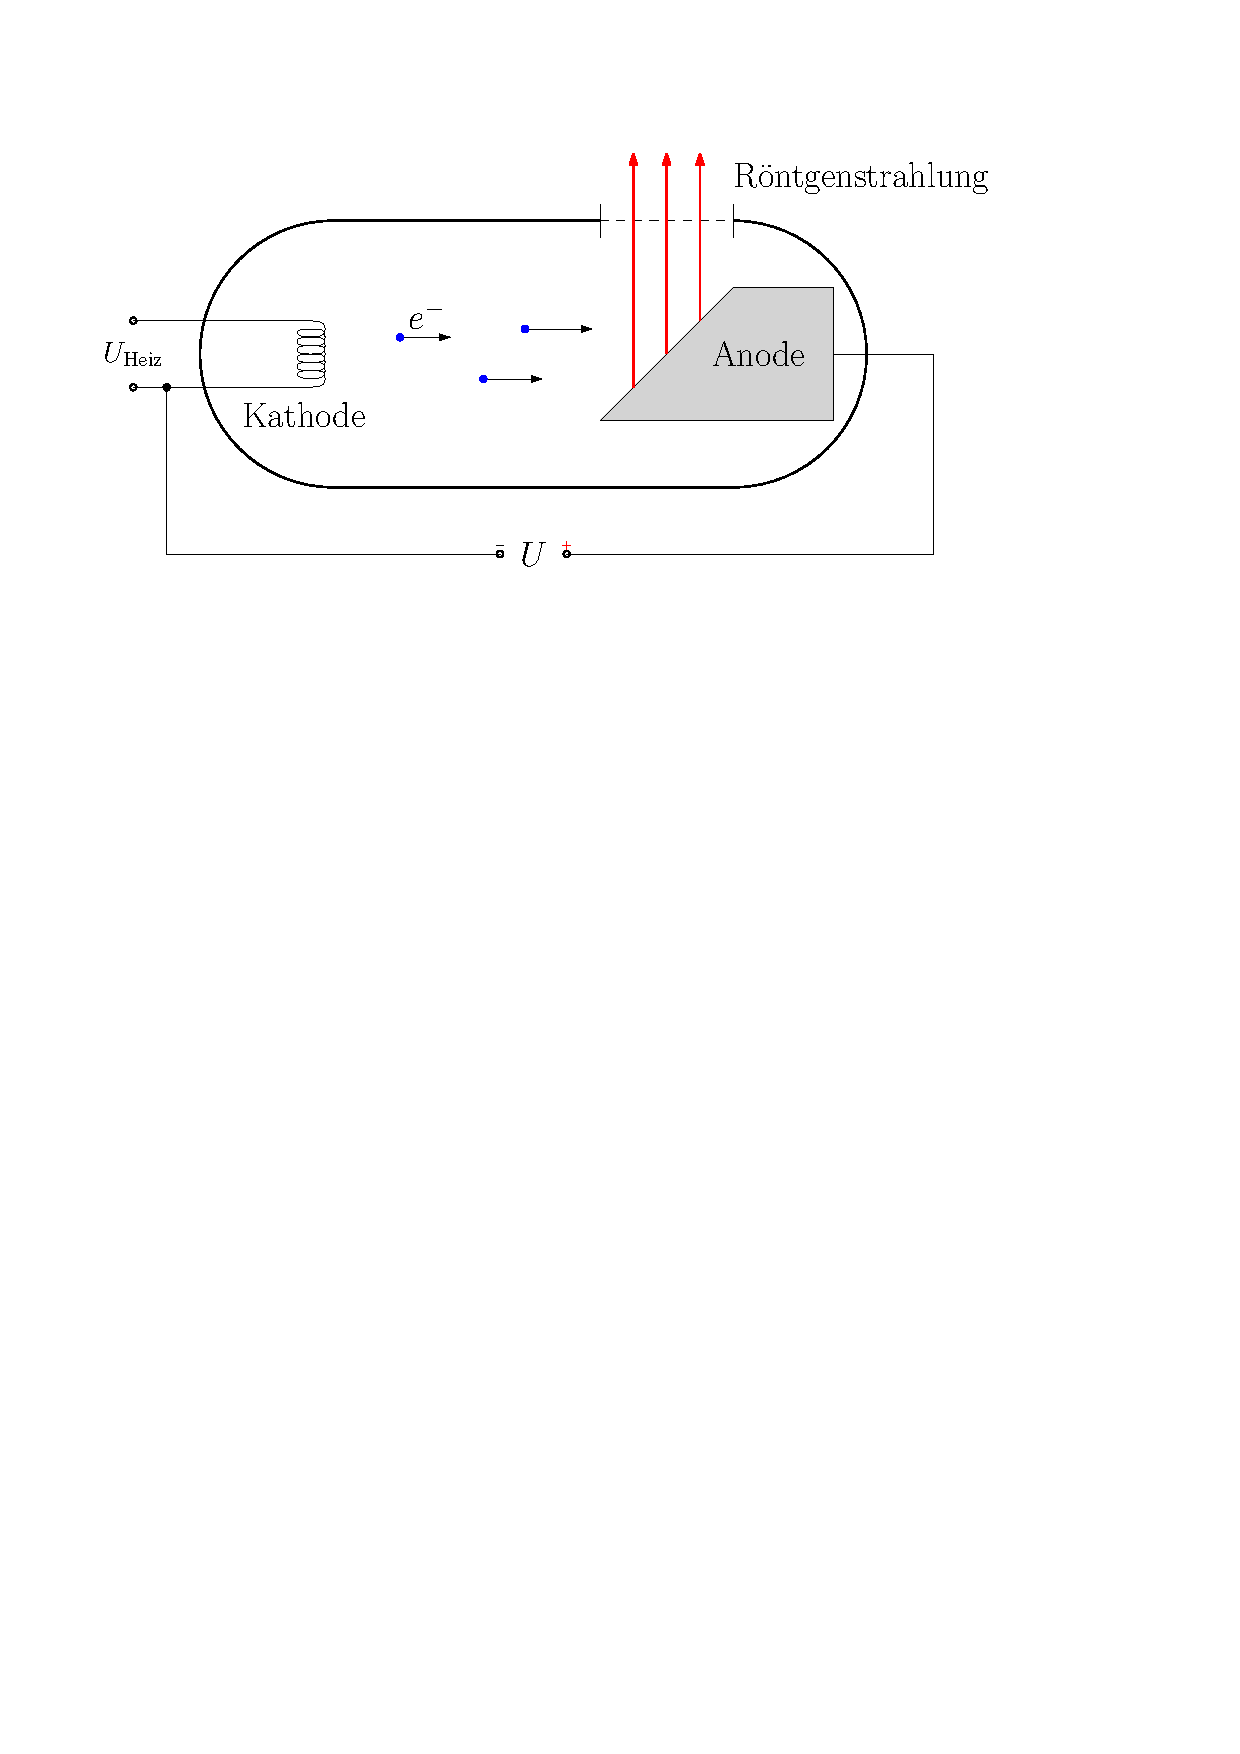
\includegraphics[width=0.75\textwidth]{./grafiken/roentgenroehre.pdf}
\caption{schematischer Aufbau einer Röntgenröhre}
\label{fig:roehre}
\end{figure}

\subsubsection{Nachweis}
Zum Nachweis von Röntgenstrahlung werden in diesem Versuch Geiger-Müller-Zählrohre, Röntgenenergiedetektor und Röntgenfilm verwendet.
Der Röntgenfilm ist mit einer speziellen Beschichtung, die bei Auftreffen von Röntgenstrahlung Licht aussendet (Schicht besser erläutern), versehen, welches wiederum eine lichtempfindliche Emulsion(?) belichtet und so ein Bild erzeugt.(Wikipedia?)
Die Funktionsweise der beiden anderen Nachweismethoden wird weiter unten erklärt.

Was noch erwähnt werden sollte:
\begin{itemize}
  \item Elektron-Loch Bildung in pn-Grenzschichten
  \item Szintillationszähler
\end{itemize}

\subsection{Bragg-Reflexion}
Betrachtet man die Beugung von einfallender elektromagnetischer Strahlung an parallelen Netzebenen eines Einkristalls, so führt die Interferenz der gebeugten Wellen zu einer Ausbildung von Beugungsmaxima.
Bezeichnet $\theta$ den Winkel des einfallenden Strahls gegen die parallelen Netzebenen (Glanzwinkel), so erhält man konstruktive Interferenz, wenn der Weglängenunterschied zwischen zwei benachbarten Netzebenen ein ganzzahliges Vielfaches der Wellenlänge $\lambda$ ist:
\begin{align}
  \Delta s = m \lambda \quad \text{für } m \in \mathbb{N}
\end{align}
Dabei ist der Weglängenunterschied gegeben durch den Netzebenenabstand $d$ und dem Glanzwinkel $\theta$:
\begin{align}
  \Delta s = 2 d \sin(\theta)
\end{align}
und man erhält die \textbf{Bedingung für Bragg-Reflexion}:
\begin{align}
  2 d \sin(\theta) = m \lambda
\end{align}

(Bild zur Veranschaulichung)

\begin{itemize}
  \item Röntgenbeugung (muss noch erklärt werden)
\end{itemize}

\subsection{Röntgenfluoreszenz}
Als Röntgenfluoreszenz bezeichnet man die Entstehung sekundärer, fluoreszierender Röntgenstrahlung.
Dies geschieht ähnlich wie die Erzeugung charakteristischer Röntgenstrahlung, nur dass nun bereits erzeugte Röntgenstrahlung anstatt den energiereichen Elektronen zur Bestrahlung eines Elements verwendet werden.
Diese sekundäre Röntgenstrahlung weist wieder ein charakteristisches Spektrum auf, aus dem man auf das beschossene Element schließen kann.
Das Verfahren zur Elementbestimmung (oder Anteilen an Elementen in dem Target (?)) nennt sich daher \textbf{Röntgenfluoreszenzanalyse}.

Aus Höhe der Linien im Count--Energie Diagramm kann Massenanteil des jeweiligen Stoffes bestimmt werden.
Höhe der Linie ist nämlich proportional zur Anzahl der strahlenden Atome.
Vergleicht man das aufgenommene Spektrum mit einem Referenzspektrum mit strahlenden Atomen:
\begin{align}
  n_0 = V \cdot \frac{\rho}{A}
\end{align}
($V$: durchstrahltes Volumen; $\rho$: Massendichte des Stoffes; $A$: Atomgewicht des Stoffes)
So kann aus der Höhe des Peaks im zu analysierenden Spektrum $H$ mit der im Referenzspektrum $H_0$ verglichen werden und daraus die Anzahl $n$ der Atome im zu analysierenden Spektrum berechnet werden:
\begin{align}
  n = n_0 \cdot \frac{H}{H_0}
\end{align}
Daher ergibt sich der Massenanteil des $i$-ten Referenzmaterials im zu analysierenden Spektrums zu:
\begin{align}
  C_i = \frac{n_i \cdot A_i}{\sum_j n_j \cdot A_j} = \frac{V \cdot \frac{\rho_i}{A_i} \cdot \frac{H_i}{H_{0,i}} \cdot A_i}{\sum_j V \cdot \frac{\rho_j}{A_j} \cdot \frac{H_j}{H_{0,j}}\cdot A_j} = \frac{\rho_i \cdot \frac{H_i}{H_{0,i}}}{\sum_j \rho_j \cdot \frac{H_j}{H_{0,j}}}
\end{align}
wobei das durchstrahlte Volumen der einzelnen Proben als gleich angenommen wurde.

\subsection{Laue-Verfahren}

\subsubsection{Elementarzelle}
Translationsvektoren mit Basis $(\vec{a}, \vec{b}, \vec{c})$

\subsubsection{Millersche Indizes}

Zur Beschreibung von Gitterebenen in einem Kristall nutzt man die s.g. Millerschen Indizes $(hkl)$, mit denen eine Gitterebene eindeutig beschrieben ist.
Man legt dabei das reale Gitter im Kristall mit den Einheitsvektoren $\vec{a}$, $\vec{b}$, $\vec{c}$ zugrunde und betrachtet die Schnittpunkte der betrachteten Gitterebene mit den jeweiligen Achsen.
Die Schnittpunkte werden dann geschrieben als S$_i=m_i\vec{e}_i$ mit $i=1,2,3$ und $\vec{e}_i= \vec{a}, \vec{b}, \vec{c}$.
Die Millerschen Indizes erhält man, wenn man die Kehrwerte $\frac{1}{m_i}$ betrachtet und $p$ so wählt, dass die reziproken Werte ganze, teilerfremde Zahlen werden\cite{demtroeder}:
\begin{align}
h=\dfrac{p}{m_1} \quad\quad k=\dfrac{p}{m_2} \quad\quad l=\dfrac{p}{m_3}
\end{align}
Betrachte dazu das Beispiel in Abbildung \ref{fig:millerindizes}:
\begin{figure}[h]
\centering
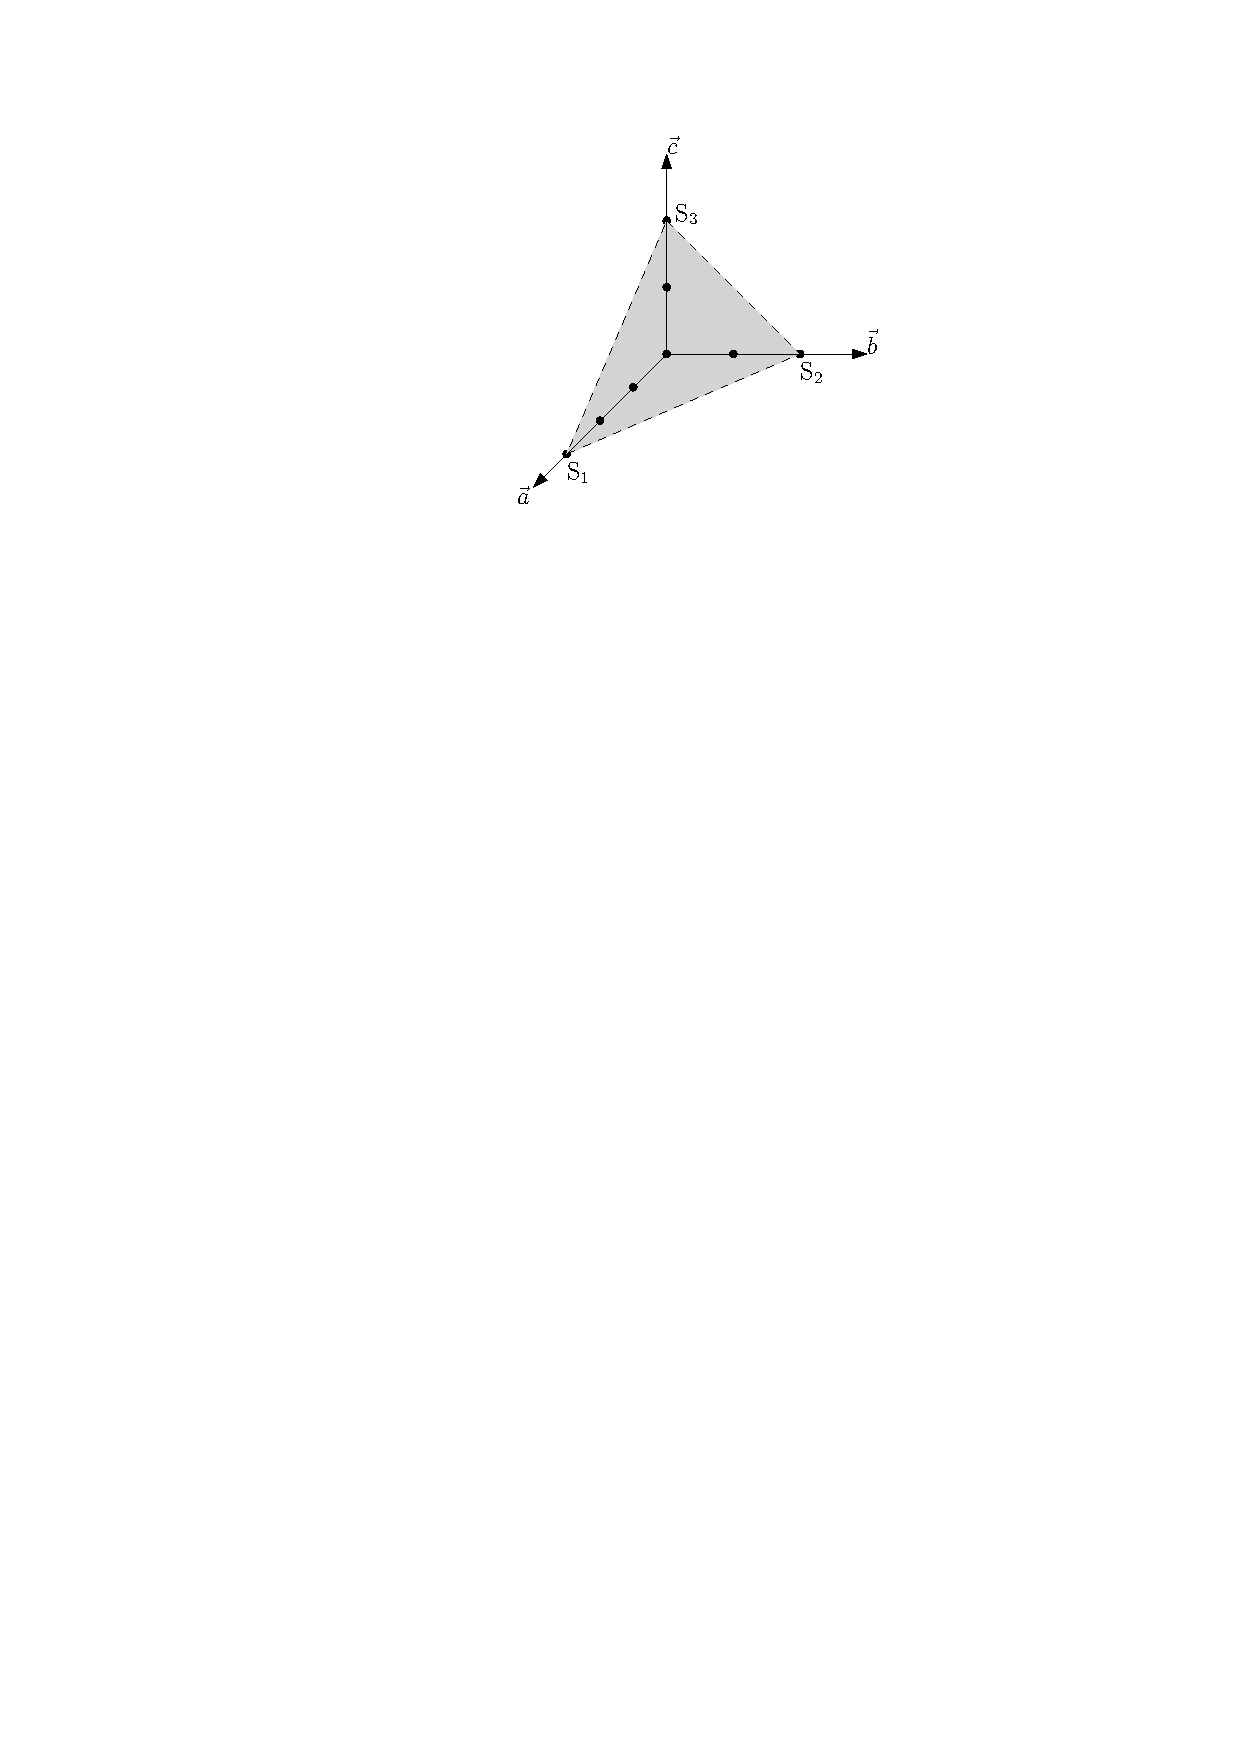
\includegraphics[width=0.4\textwidth]{./grafiken/millerindizes.pdf}
\caption{Beispiel zur Bestimmung der Millerindizes mit $m_1=3$, $m_2=2$, $m_3=2$. Die Ebene wird dann beschrieben durch $(233)$ (mit $p=6$).}
\label{fig:millerindizes}
\end{figure}

\subsubsection{reziprokes Gitter}
Definiert anhand der Basisvektoren des Gitters (demtröder):

\begin{align}
  \vec{a}^{*} = \frac{2\pi}{V_\mathrm{E}} \cdot ( \vec{b} \times \vec{c} ) \nonumber\\
  \vec{b}^{*} = \frac{2\pi}{V_\mathrm{E}} \cdot ( \vec{c} \times \vec{a} ) \nonumber\\
  \vec{c}^{*} = \frac{2\pi}{V_\mathrm{E}} \cdot ( \vec{a} \times \vec{b} )
\end{align}
Mit dem Volumen der Elementarzelle
\begin{align}
  V_\mathrm{E} = \vec{a} \cdot \left( b \times c \right)
\end{align}
Besondere Zusammenhänge mit den durch die millersche Indizes $(hkl)$ ausgezeichnete Ebenenschar:
\begin{align}
  \vec{G} = h \vec{a}^{*} + k \vec{b}^{*} + l \vec{c}^{*}
\end{align}
steht senkrecht auf der Ebenenschar $(hkl)$.
\begin{align}
  | \vec{G} | = \frac{2\pi}{d_{hkl}}
\end{align}
wobei $d_{hkl}$ der Abstand zweier benachbarter Ebenen ist.



\begin{itemize}
  \item Laue--Bedingung
  \item Millersche Indizes (reziprokes Gitter)
  \item Elementarzelle
  \item Glanzwinkel
  \item Netzebenenabstand
\end{itemize}

\subsection{Geiger-Müller-Zählrohr}

Das Geiger-Müller-Zählrohr besteht aus einem Metallzylinder, der die Kathode darstellt und einem Draht im Inneren des Zylinders, der die Anode bildet.
Der Zylinder ist mit einem Gas unter hohem Druck gefüllt, wobei meistens Edelgas verwendet wird, da diese keinen negativen Ionen bilden, die den Betrieb stören können.
Bei Eintritt von Teilchen in das Zählrohr werden die Gasatome ionisiert und so freie Elektronen erzeugt.
Durch die zwischen Draht und Zylindermantel anliegende Spannung werden diese zum Draht beschleunigt.
Dadurch entsteht ein Stromimpuls, der dann an einem digitalen Zähler registriert wird, wobei die Anzahl Elektronen bei geladenen zu zählenden Teilchen und damit die Anzahl Impulse der Anzahl der einfallenden Teilchen entspricht.
Für den Betrieb ist die angelegte Gleichspannung zwischen Anode und Kathode entscheidend.
Bei zu geringer Spannung können die freien Elektronen auf der Beschleunigungstrecke wieder mit den Gasatomen rekombinieren (Rekombinationsbereich), wodurch die Messung verfälscht wird.
Erst ab einer bestimmten Gleichspannung erreichen alle Elektronen die Anode, womit dann die von der Strahlung im Zählrohr abgegebene Energie gemessen wird.
Beim Geiger-Müller-Zählrohr ist das Zählrohr so ausgelegt, dass die Elektronen durch die Beschleunigung Energien erreichen, die zur weiteren Ionisation der Gasatome führen, wodurch sich ein s.g. Lawineneffekt einstellt.

\begin{itemize}
  \item Aufbau
  \item Funktionsweise
  \item Totzeit
\end{itemize}

\subsection{Röntgenenergiedetektor}
\textbf{Aufbau:} PIN-Photodiode ($Q \propto E_\gamma$) -- Charge Amplifier (Integrator $U_\mathrm{out} \propto \int I = Q$) -- Verstärkerstufe ($U = V \cdot U_\mathrm{out}$)
Außerdem Kühlnug der PIN-Diode um den Leckstrom zu verringern (hier Peltier-Effekt)

\textbf{PIN-Photodiode:} Besteht aus einer PIN-Halbleiterschicht, wobei I für intrinischem Halbleiter (undotiert) steht.
Unter reverse Bias bildet sich eine Verarmungszone im intrinsischen Halbleiterbereich.
Wird ein Röntgenphoton in der intrinsischen Zone absorbiert (Photoeffekt) und löst ein Elektron aus den Halbleiteratomen, sodass ein Elektron-Loch Paar entsteht.
Das hochenergetische Elektron kann nun weitere Kristallatome ionisieren oder auch unter Ausstrahlung eines charakteristischen Röntgenphotons erneut ein Elektron-Loch Paar erzeugen.
Dies passiert sooft, bis die gesamte Energie des Röntgenphotons in Elektronen-Loch Paare umgewandelt wurde, deren Anzahl gegeben ist durch:
\begin{align}
  N = \frac{E_\gamma}{W_{e,\mathrm{Loch}}}
\end{align}
Dadurch entsteht ein Ladungsfluss proportional zur Energie des Röntgenquants.

\textbf{Funktionsweise:} Dieser Strom kann wird in einem Integrator (Op amp?) aufintegriert um die Gesamtladung zu erhalten.
Diese wird wiederum in einer nächsten Verstärkerstufe verstärkt, um eine zur Photonenenergie proportionale Spannung zu erhalten.

\textbf{Vielkanalanalysator:} Ein DAC die zur Photonenenergie proportionale (verstärkte) Spannung $U$ in einen digitalen Wert um, sodass aufgrund der endlichen Auflösung des DAC's die Energien in Bins (Histogram!) deren Breite durch das Auflösungsvermögen gegeben sind.
Mit jedem Impuls (Photondetektion) wird der zu dem digitalen Wert gehörende Bin um eins hochgezählt.

\textbf{Kalibrierung:} Aufgrund der unbekannten Proportionalitäten und Nullpunktsverschiebung muss die Energie anhand von zwei Kalibrationswerten
(Bestimmung von m und b) bestimmt werden.
\begin{align}
  E = m \cdot U_\mathrm{digital} + b
\end{align}

\section{Bragg-Reflekion}
Im Folgenden wollen wir unter Ausnutzung von Bragg-Reflektion an einem NaCl-Einkristall die Wellenlänge und Energie des charakteristischen Röntgenspektrums einer unbekannten Röhrenanode bestimmen und anhand dessen das Anodenmaterial bestimmen.
Anschließend wird die Feinstrukturaufspaltung $\Delta \lambda$ der $K_\alpha$-Linie der charakteristischen Röntgenstrahlung einer Molybdän-Anode in vierter Beugungsordnung bestimmt.

\subsection{Versuchsdurchführung}
\subsubsection{Bestimmung der charakteristischen Röntgenstrahlung einer unbekannten Röhre}
\begin{figure}[h]
\centering
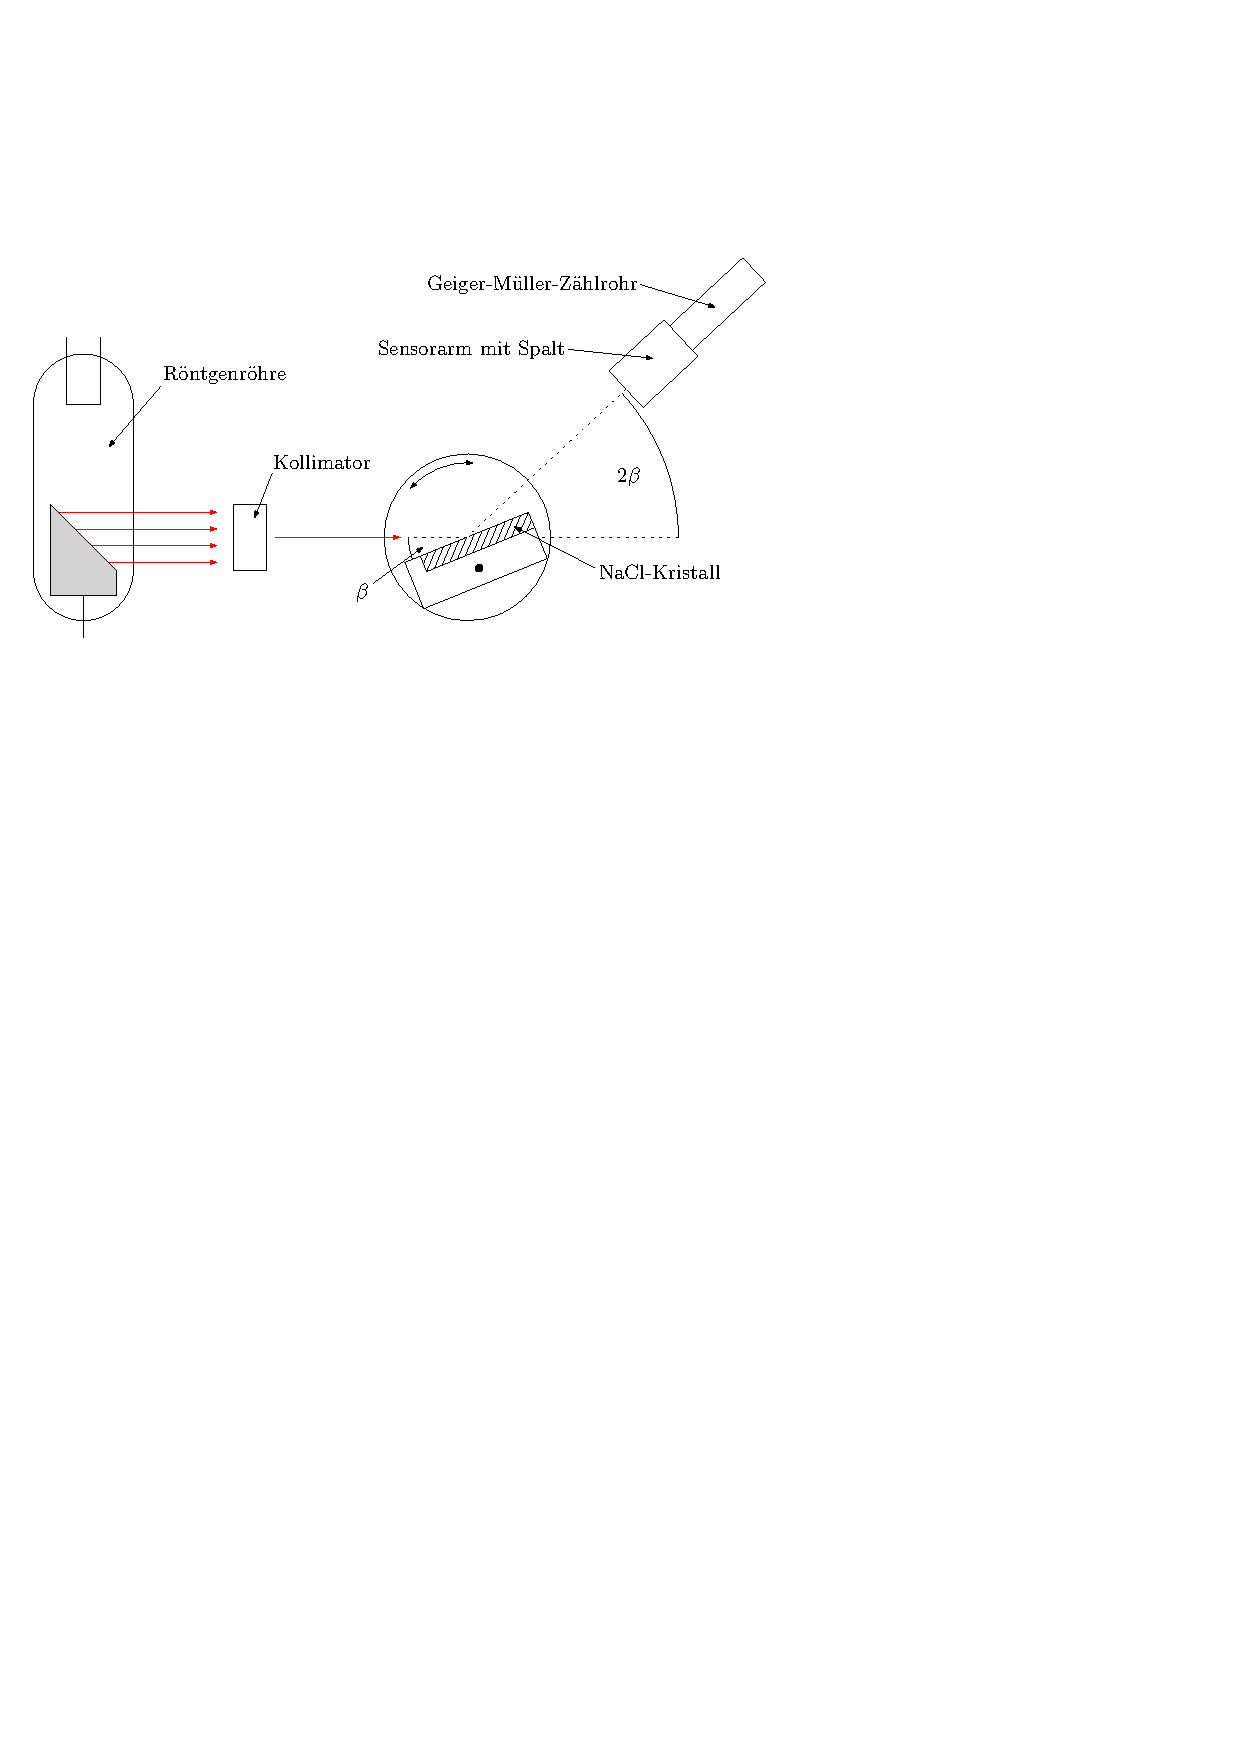
\includegraphics[width=0.9\textwidth]{./grafiken/aufbau_bragg.pdf}
\caption{Versuchsaufbau zur Bragg-Reflektion am NaCl-Kristall}
\label{fig:bragg_aufbau}
\end{figure}
Zur Aufnahme des charakteristischen Röntgenspektrums einer unbekannten Anode wird das Vollschutzröntgengerät verwendet, dessen innerer Aufbau in Abbildung \ref{fig:bragg_aufbau} dargestellt ist.
Zunächst tauschen wir die installierte Röntgenröhre gegen die \textbf{unbekannte Röntgenröhre 3} aus.
Zur Kollimation der Röntgenstrahlung der Röntgenröhre verwenden wir den Kollimatorspalt der Breite \SI{1}{\milli\metre}, welcher in den vorgesehenen Sockel des Vollschutzröntgengeräts eingesetzt wird.
Dies ist nötig, da die Röntgenstrahlung nicht parallel aus der Röntgenröhre austritt und daher ohne Kollimation kein scharfes Spektrum entsteht, da die Strahlen unter verschiedenen Glanzwinkeln auf das Target treffen.

Im Experimentierraum des Röntgengeräts befindet sich das Goniometer, an welchem zunächst der Sensorarm mit \SI{1}{\milli\metre} Spalt befestigt wird.
In diesen setzen wir das Geiger-Müller-Zählrohr ein, (anschließen an die Elektronik).
Schließlich wird der Targettisch an dem Goniometer befestigt und der NaCl-Kristall so auf dem Tisch befestigt, dass dessen Rotationsachse etwa auf der Kristalloberfläche liegt.
Dabei wurden Sensorarm und Goniometer so positioniert, dass der Abstand Kollimatorspalt--Target und Sensorarm--Target \num{5} bis \SI{6}{\centi\metre} beträgt.
Das Goniometer dient nun zur computergesteuerten Einstellung der Winkel von Targettisch $\beta_\mathrm{Target}$ und Sensorarm $\beta_\mathrm{Sensor}$ zur Horizontalen.
Da bei Bragg-Reflektion der Winkel des einfallenden Strahls zum Target gleich dem des Ausfallenden ist, wird das Goniometer im \emph{Coupled}-Modus betrieben, welcher das Target und den Sensorarm stets so einstellt, dass die Bedingung $\beta = \beta_\mathrm{Target} = 2\beta_\mathrm{Sensor}$ erfüllt ist.

Die eigentliche Messung wird nun computergesteuert durchgeführt.
Dabei verwenden wir eine Röhrenspannung von \SI{35}{\kilo\volt} mit einem Emissionsstrom zwischen Glühkathode und Anode von \SI{1}{\milli\ampere}.
Wir vermessen einen Glanzwinkelbereich von $\beta_\mathrm{min} = \SI{2,0}{\degree}$ bis $\beta_\mathrm{max} = \SI{25,0}{\degree}$ in Schritten von $\Delta \beta = \SI{0,1}{\degree}$, wobei jede Winkeleinstellung für $\Delta t = \SI{10}{\second}$ gehalten wird und die mittlere Zählrate des Zählrohrs über dem Zeitintervall durch das Programm gemessen wird.

Nach dem Abschluss der Messung wurde das Spektrum mithilfe der Funktion \emph{'Peakschwerpunkt berechnen'} des Programmes ausgemessen. Auf die genaue Vorgehensweise wird dabei in der Auswertung eingegangen.

\subsubsection{Bestimmung der Feinstruktur der $K_\alpha$-Linie von Molybdän}



\subsection{Messdaten}

\begin{table}[h]
\centering
\begin{tabular}{lSScSS}
\toprule
{Peaknummer} & {Winkel $\beta / \si{\degree}$} & {Fehler $\Delta\beta / \si{\degree}$} & Ordnung & {Energie $E / \si{\electronvolt}$} & {Fehler $\Delta E / \si{\electronvolt}$}\\
\midrule
1&	11.047&	0.213&	1	&	11495.6&	218.9 \\
2&	12.919&	0.259&	1	&	9852.3&	194.2\\
3&	15.108&	0.148&	1	&	8451.2&	80.9\\
4&	17.242&	0.135&		&	7431.4&	56.4\\
5&	20.023&	0.101&		&	6433.2&	31.1\\
6&	22.037&	0.099&	2	&	5870.7&	25.1\\
7&	22.780&	0.104&	2	&	5688.9&	24.6\\
\bottomrule
\end{tabular}
\caption{Peakschwerpunkte in der Grobstruktur der unbekannten Anode und Umrechnung in die entsprechende Energie}
\label{fig:peakschwerpunkt_grobstruktur}
\end{table}

\begin{table}[h]
\centering
\begin{tabular}{lSS}
\toprule
{\#} & {$\beta_\mathrm{Peak} / \si{\degree}$} & {$\sigma_\beta / \si{\degree}$} \\
\midrule
1&	30.1827&	0.0200 \\
2&	30.3824&	0.0205 \\
\bottomrule
\end{tabular}
\caption{Peakschwerpunkte in der Feinstruktur der Molybdänanode (in vierter Ordnung)}
\label{fig:peakschwerpunkt_feinstruktur}
\end{table}

\begin{figure}[h]
\centering
% GNUPLOT: LaTeX picture with Postscript
\begingroup
  \makeatletter
  \providecommand\color[2][]{%
    \GenericError{(gnuplot) \space\space\space\@spaces}{%
      Package color not loaded in conjunction with
      terminal option `colourtext'%
    }{See the gnuplot documentation for explanation.%
    }{Either use 'blacktext' in gnuplot or load the package
      color.sty in LaTeX.}%
    \renewcommand\color[2][]{}%
  }%
  \providecommand\includegraphics[2][]{%
    \GenericError{(gnuplot) \space\space\space\@spaces}{%
      Package graphicx or graphics not loaded%
    }{See the gnuplot documentation for explanation.%
    }{The gnuplot epslatex terminal needs graphicx.sty or graphics.sty.}%
    \renewcommand\includegraphics[2][]{}%
  }%
  \providecommand\rotatebox[2]{#2}%
  \@ifundefined{ifGPcolor}{%
    \newif\ifGPcolor
    \GPcolortrue
  }{}%
  \@ifundefined{ifGPblacktext}{%
    \newif\ifGPblacktext
    \GPblacktexttrue
  }{}%
  % define a \g@addto@macro without @ in the name:
  \let\gplgaddtomacro\g@addto@macro
  % define empty templates for all commands taking text:
  \gdef\gplbacktext{}%
  \gdef\gplfronttext{}%
  \makeatother
  \ifGPblacktext
    % no textcolor at all
    \def\colorrgb#1{}%
    \def\colorgray#1{}%
  \else
    % gray or color?
    \ifGPcolor
      \def\colorrgb#1{\color[rgb]{#1}}%
      \def\colorgray#1{\color[gray]{#1}}%
      \expandafter\def\csname LTw\endcsname{\color{white}}%
      \expandafter\def\csname LTb\endcsname{\color{black}}%
      \expandafter\def\csname LTa\endcsname{\color{black}}%
      \expandafter\def\csname LT0\endcsname{\color[rgb]{1,0,0}}%
      \expandafter\def\csname LT1\endcsname{\color[rgb]{0,1,0}}%
      \expandafter\def\csname LT2\endcsname{\color[rgb]{0,0,1}}%
      \expandafter\def\csname LT3\endcsname{\color[rgb]{1,0,1}}%
      \expandafter\def\csname LT4\endcsname{\color[rgb]{0,1,1}}%
      \expandafter\def\csname LT5\endcsname{\color[rgb]{1,1,0}}%
      \expandafter\def\csname LT6\endcsname{\color[rgb]{0,0,0}}%
      \expandafter\def\csname LT7\endcsname{\color[rgb]{1,0.3,0}}%
      \expandafter\def\csname LT8\endcsname{\color[rgb]{0.5,0.5,0.5}}%
    \else
      % gray
      \def\colorrgb#1{\color{black}}%
      \def\colorgray#1{\color[gray]{#1}}%
      \expandafter\def\csname LTw\endcsname{\color{white}}%
      \expandafter\def\csname LTb\endcsname{\color{black}}%
      \expandafter\def\csname LTa\endcsname{\color{black}}%
      \expandafter\def\csname LT0\endcsname{\color{black}}%
      \expandafter\def\csname LT1\endcsname{\color{black}}%
      \expandafter\def\csname LT2\endcsname{\color{black}}%
      \expandafter\def\csname LT3\endcsname{\color{black}}%
      \expandafter\def\csname LT4\endcsname{\color{black}}%
      \expandafter\def\csname LT5\endcsname{\color{black}}%
      \expandafter\def\csname LT6\endcsname{\color{black}}%
      \expandafter\def\csname LT7\endcsname{\color{black}}%
      \expandafter\def\csname LT8\endcsname{\color{black}}%
    \fi
  \fi
  \setlength{\unitlength}{0.0500bp}%
  \begin{picture}(7200.00,4320.00)%
    \gplgaddtomacro\gplbacktext{%
      \csname LTb\endcsname%
      \put(1078,704){\makebox(0,0)[r]{\strut{} 0}}%
      \csname LTb\endcsname%
      \put(1078,1295){\makebox(0,0)[r]{\strut{} 500}}%
      \csname LTb\endcsname%
      \put(1078,1886){\makebox(0,0)[r]{\strut{} 1000}}%
      \csname LTb\endcsname%
      \put(1078,2477){\makebox(0,0)[r]{\strut{} 1500}}%
      \csname LTb\endcsname%
      \put(1078,3068){\makebox(0,0)[r]{\strut{} 2000}}%
      \csname LTb\endcsname%
      \put(1078,3659){\makebox(0,0)[r]{\strut{} 2500}}%
      \csname LTb\endcsname%
      \put(1210,484){\makebox(0,0){\strut{} 0}}%
      \csname LTb\endcsname%
      \put(2329,484){\makebox(0,0){\strut{} 5}}%
      \csname LTb\endcsname%
      \put(3447,484){\makebox(0,0){\strut{} 10}}%
      \csname LTb\endcsname%
      \put(4566,484){\makebox(0,0){\strut{} 15}}%
      \csname LTb\endcsname%
      \put(5684,484){\makebox(0,0){\strut{} 20}}%
      \csname LTb\endcsname%
      \put(6803,484){\makebox(0,0){\strut{} 25}}%
      \put(176,2181){\rotatebox{-270}{\makebox(0,0){\strut{}Z\"ahlrate}}}%
      \put(4006,154){\makebox(0,0){\strut{}Glanzwinkel $\theta$ / \si{\degree}}}%
      \put(4006,3989){\makebox(0,0){\strut{}Gemessene Z\"ahlrate für unterschiedliche Winkel bei Bragg-Beugung}}%
    }%
    \gplgaddtomacro\gplfronttext{%
      \csname LTb\endcsname%
      \put(5816,3486){\makebox(0,0)[r]{\strut{}Zählrate}}%
    }%
    \gplbacktext
    \put(0,0){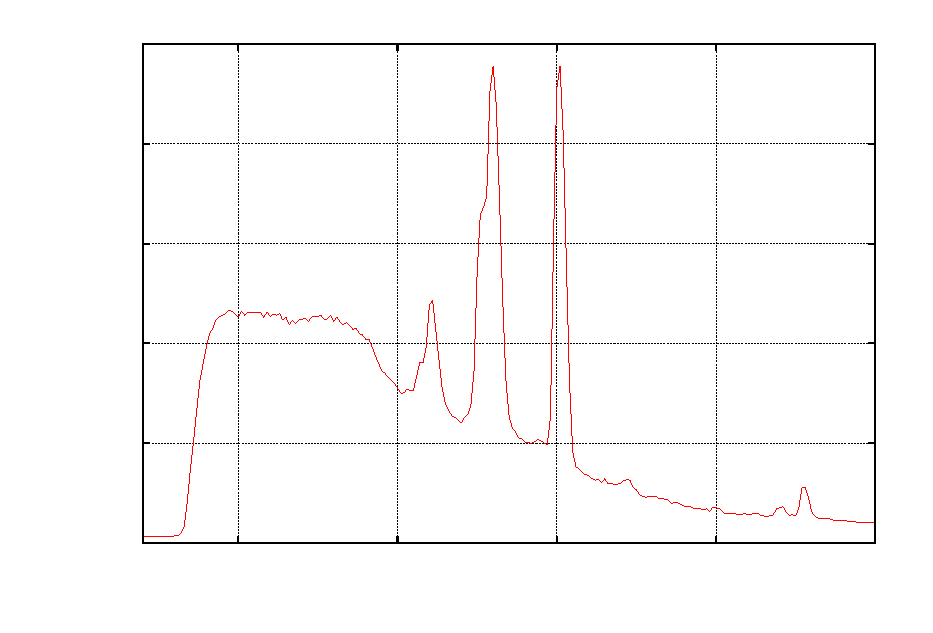
\includegraphics{./plots/anode3}}%
    \gplfronttext
  \end{picture}%
\endgroup

\caption{Aufgenommenes Röntgenspektrum der unbekannten Anode bei Bragg-Streuung an einem NaCl-Kristall}
\label{fig:anode3}
\end{figure}

\subsection{Auswertung}


\subsection{Diskussion}

\section{Zerstörungsfreie Analyse chemischer Zusammensetzungen}
\subsection{Versuchsdurchführung}
\subsection{Messdaten}
\subsection{Auswertung}
\subsection{Diskussion}

\section{Laue-Aufnahme}
\subsection{Versuchsdurchführung}
\subsection{Messdaten}
\subsection{Auswertung}
\subsection{Diskussion}


\section{Zusammenfassung}

\begin{figure}
\centering
% GNUPLOT: LaTeX picture with Postscript
\begingroup
  \makeatletter
  \providecommand\color[2][]{%
    \GenericError{(gnuplot) \space\space\space\@spaces}{%
      Package color not loaded in conjunction with
      terminal option `colourtext'%
    }{See the gnuplot documentation for explanation.%
    }{Either use 'blacktext' in gnuplot or load the package
      color.sty in LaTeX.}%
    \renewcommand\color[2][]{}%
  }%
  \providecommand\includegraphics[2][]{%
    \GenericError{(gnuplot) \space\space\space\@spaces}{%
      Package graphicx or graphics not loaded%
    }{See the gnuplot documentation for explanation.%
    }{The gnuplot epslatex terminal needs graphicx.sty or graphics.sty.}%
    \renewcommand\includegraphics[2][]{}%
  }%
  \providecommand\rotatebox[2]{#2}%
  \@ifundefined{ifGPcolor}{%
    \newif\ifGPcolor
    \GPcolortrue
  }{}%
  \@ifundefined{ifGPblacktext}{%
    \newif\ifGPblacktext
    \GPblacktexttrue
  }{}%
  % define a \g@addto@macro without @ in the name:
  \let\gplgaddtomacro\g@addto@macro
  % define empty templates for all commands taking text:
  \gdef\gplbacktext{}%
  \gdef\gplfronttext{}%
  \makeatother
  \ifGPblacktext
    % no textcolor at all
    \def\colorrgb#1{}%
    \def\colorgray#1{}%
  \else
    % gray or color?
    \ifGPcolor
      \def\colorrgb#1{\color[rgb]{#1}}%
      \def\colorgray#1{\color[gray]{#1}}%
      \expandafter\def\csname LTw\endcsname{\color{white}}%
      \expandafter\def\csname LTb\endcsname{\color{black}}%
      \expandafter\def\csname LTa\endcsname{\color{black}}%
      \expandafter\def\csname LT0\endcsname{\color[rgb]{1,0,0}}%
      \expandafter\def\csname LT1\endcsname{\color[rgb]{0,1,0}}%
      \expandafter\def\csname LT2\endcsname{\color[rgb]{0,0,1}}%
      \expandafter\def\csname LT3\endcsname{\color[rgb]{1,0,1}}%
      \expandafter\def\csname LT4\endcsname{\color[rgb]{0,1,1}}%
      \expandafter\def\csname LT5\endcsname{\color[rgb]{1,1,0}}%
      \expandafter\def\csname LT6\endcsname{\color[rgb]{0,0,0}}%
      \expandafter\def\csname LT7\endcsname{\color[rgb]{1,0.3,0}}%
      \expandafter\def\csname LT8\endcsname{\color[rgb]{0.5,0.5,0.5}}%
    \else
      % gray
      \def\colorrgb#1{\color{black}}%
      \def\colorgray#1{\color[gray]{#1}}%
      \expandafter\def\csname LTw\endcsname{\color{white}}%
      \expandafter\def\csname LTb\endcsname{\color{black}}%
      \expandafter\def\csname LTa\endcsname{\color{black}}%
      \expandafter\def\csname LT0\endcsname{\color{black}}%
      \expandafter\def\csname LT1\endcsname{\color{black}}%
      \expandafter\def\csname LT2\endcsname{\color{black}}%
      \expandafter\def\csname LT3\endcsname{\color{black}}%
      \expandafter\def\csname LT4\endcsname{\color{black}}%
      \expandafter\def\csname LT5\endcsname{\color{black}}%
      \expandafter\def\csname LT6\endcsname{\color{black}}%
      \expandafter\def\csname LT7\endcsname{\color{black}}%
      \expandafter\def\csname LT8\endcsname{\color{black}}%
    \fi
  \fi
  \setlength{\unitlength}{0.0500bp}%
  \begin{picture}(8640.00,12960.00)%
      \csname LTb\endcsname%
      \put(4320,12740){\makebox(0,0){\strut{}Referenzspektren Teil 1}}%
    \gplgaddtomacro\gplbacktext{%
      \csname LTb\endcsname%
      \put(732,8748){\makebox(0,0)[r]{\strut{}0}}%
      \csname LTb\endcsname%
      \put(732,9461){\makebox(0,0)[r]{\strut{}2000}}%
      \csname LTb\endcsname%
      \put(732,10173){\makebox(0,0)[r]{\strut{}4000}}%
      \csname LTb\endcsname%
      \put(732,10886){\makebox(0,0)[r]{\strut{}6000}}%
      \csname LTb\endcsname%
      \put(732,11598){\makebox(0,0)[r]{\strut{}8000}}%
      \csname LTb\endcsname%
      \put(732,12311){\makebox(0,0)[r]{\strut{}10000}}%
      \csname LTb\endcsname%
      \put(864,8528){\makebox(0,0){\strut{} }}%
      \csname LTb\endcsname%
      \put(1540,8528){\makebox(0,0){\strut{} }}%
      \csname LTb\endcsname%
      \put(2216,8528){\makebox(0,0){\strut{} }}%
      \csname LTb\endcsname%
      \put(2892,8528){\makebox(0,0){\strut{} }}%
      \csname LTb\endcsname%
      \put(3569,8528){\makebox(0,0){\strut{} }}%
      \csname LTb\endcsname%
      \put(4245,8528){\makebox(0,0){\strut{} }}%
      \put(-170,10529){\rotatebox{-270}{\makebox(0,0){\strut{}Counts}}}%
      \put(4043,12026){\makebox(0,0)[l]{\strut{}Pb}}%
    }%
    \gplgaddtomacro\gplfronttext{%
    }%
    \gplgaddtomacro\gplbacktext{%
      \csname LTb\endcsname%
      \put(4188,8748){\makebox(0,0)[r]{\strut{}}}%
      \csname LTb\endcsname%
      \put(4188,9461){\makebox(0,0)[r]{\strut{}}}%
      \csname LTb\endcsname%
      \put(4188,10173){\makebox(0,0)[r]{\strut{}}}%
      \csname LTb\endcsname%
      \put(4188,10886){\makebox(0,0)[r]{\strut{}}}%
      \csname LTb\endcsname%
      \put(4188,11598){\makebox(0,0)[r]{\strut{}}}%
      \csname LTb\endcsname%
      \put(4188,12311){\makebox(0,0)[r]{\strut{}}}%
      \csname LTb\endcsname%
      \put(4320,8528){\makebox(0,0){\strut{} }}%
      \csname LTb\endcsname%
      \put(4996,8528){\makebox(0,0){\strut{} }}%
      \csname LTb\endcsname%
      \put(5672,8528){\makebox(0,0){\strut{} }}%
      \csname LTb\endcsname%
      \put(6348,8528){\makebox(0,0){\strut{} }}%
      \csname LTb\endcsname%
      \put(7025,8528){\makebox(0,0){\strut{} }}%
      \csname LTb\endcsname%
      \put(7701,8528){\makebox(0,0){\strut{} }}%
      \put(7499,12026){\makebox(0,0)[l]{\strut{}Fe}}%
    }%
    \gplgaddtomacro\gplfronttext{%
    }%
    \gplgaddtomacro\gplbacktext{%
      \csname LTb\endcsname%
      \put(732,4860){\makebox(0,0)[r]{\strut{}0}}%
      \csname LTb\endcsname%
      \put(732,5573){\makebox(0,0)[r]{\strut{}2000}}%
      \csname LTb\endcsname%
      \put(732,6285){\makebox(0,0)[r]{\strut{}4000}}%
      \csname LTb\endcsname%
      \put(732,6998){\makebox(0,0)[r]{\strut{}6000}}%
      \csname LTb\endcsname%
      \put(732,7710){\makebox(0,0)[r]{\strut{}8000}}%
      \csname LTb\endcsname%
      \put(732,8423){\makebox(0,0)[r]{\strut{}10000}}%
      \csname LTb\endcsname%
      \put(864,4640){\makebox(0,0){\strut{} }}%
      \csname LTb\endcsname%
      \put(1540,4640){\makebox(0,0){\strut{} }}%
      \csname LTb\endcsname%
      \put(2216,4640){\makebox(0,0){\strut{} }}%
      \csname LTb\endcsname%
      \put(2892,4640){\makebox(0,0){\strut{} }}%
      \csname LTb\endcsname%
      \put(3569,4640){\makebox(0,0){\strut{} }}%
      \csname LTb\endcsname%
      \put(4245,4640){\makebox(0,0){\strut{} }}%
      \put(-170,6641){\rotatebox{-270}{\makebox(0,0){\strut{}Counts}}}%
      \put(4043,8138){\makebox(0,0)[l]{\strut{}Au}}%
    }%
    \gplgaddtomacro\gplfronttext{%
    }%
    \gplgaddtomacro\gplbacktext{%
      \csname LTb\endcsname%
      \put(4188,4860){\makebox(0,0)[r]{\strut{}}}%
      \csname LTb\endcsname%
      \put(4188,5573){\makebox(0,0)[r]{\strut{}}}%
      \csname LTb\endcsname%
      \put(4188,6285){\makebox(0,0)[r]{\strut{}}}%
      \csname LTb\endcsname%
      \put(4188,6998){\makebox(0,0)[r]{\strut{}}}%
      \csname LTb\endcsname%
      \put(4188,7710){\makebox(0,0)[r]{\strut{}}}%
      \csname LTb\endcsname%
      \put(4188,8423){\makebox(0,0)[r]{\strut{}}}%
      \csname LTb\endcsname%
      \put(4320,4640){\makebox(0,0){\strut{} }}%
      \csname LTb\endcsname%
      \put(4996,4640){\makebox(0,0){\strut{} }}%
      \csname LTb\endcsname%
      \put(5672,4640){\makebox(0,0){\strut{} }}%
      \csname LTb\endcsname%
      \put(6348,4640){\makebox(0,0){\strut{} }}%
      \csname LTb\endcsname%
      \put(7025,4640){\makebox(0,0){\strut{} }}%
      \csname LTb\endcsname%
      \put(7701,4640){\makebox(0,0){\strut{} }}%
      \put(7499,8138){\makebox(0,0)[l]{\strut{}In}}%
    }%
    \gplgaddtomacro\gplfronttext{%
    }%
    \gplgaddtomacro\gplbacktext{%
      \csname LTb\endcsname%
      \put(732,971){\makebox(0,0)[r]{\strut{}0}}%
      \csname LTb\endcsname%
      \put(732,1684){\makebox(0,0)[r]{\strut{}2000}}%
      \csname LTb\endcsname%
      \put(732,2397){\makebox(0,0)[r]{\strut{}4000}}%
      \csname LTb\endcsname%
      \put(732,3109){\makebox(0,0)[r]{\strut{}6000}}%
      \csname LTb\endcsname%
      \put(732,3822){\makebox(0,0)[r]{\strut{}8000}}%
      \csname LTb\endcsname%
      \put(732,4535){\makebox(0,0)[r]{\strut{}10000}}%
      \csname LTb\endcsname%
      \put(864,751){\makebox(0,0){\strut{} }}%
      \csname LTb\endcsname%
      \put(1540,751){\makebox(0,0){\strut{} }}%
      \csname LTb\endcsname%
      \put(2216,751){\makebox(0,0){\strut{} }}%
      \csname LTb\endcsname%
      \put(2892,751){\makebox(0,0){\strut{} }}%
      \csname LTb\endcsname%
      \put(3569,751){\makebox(0,0){\strut{} }}%
      \csname LTb\endcsname%
      \put(4245,751){\makebox(0,0){\strut{} }}%
      \put(-170,2753){\rotatebox{-270}{\makebox(0,0){\strut{}Counts}}}%
      \put(2591,421){\makebox(0,0){\strut{}x}}%
      \put(4043,4250){\makebox(0,0)[l]{\strut{}Cu}}%
    }%
    \gplgaddtomacro\gplfronttext{%
    }%
    \gplgaddtomacro\gplbacktext{%
      \csname LTb\endcsname%
      \put(4188,971){\makebox(0,0)[r]{\strut{}}}%
      \csname LTb\endcsname%
      \put(4188,1684){\makebox(0,0)[r]{\strut{}}}%
      \csname LTb\endcsname%
      \put(4188,2397){\makebox(0,0)[r]{\strut{}}}%
      \csname LTb\endcsname%
      \put(4188,3109){\makebox(0,0)[r]{\strut{}}}%
      \csname LTb\endcsname%
      \put(4188,3822){\makebox(0,0)[r]{\strut{}}}%
      \csname LTb\endcsname%
      \put(4188,4535){\makebox(0,0)[r]{\strut{}}}%
      \csname LTb\endcsname%
      \put(4320,751){\makebox(0,0){\strut{} }}%
      \csname LTb\endcsname%
      \put(4996,751){\makebox(0,0){\strut{} }}%
      \csname LTb\endcsname%
      \put(5672,751){\makebox(0,0){\strut{} }}%
      \csname LTb\endcsname%
      \put(6348,751){\makebox(0,0){\strut{} }}%
      \csname LTb\endcsname%
      \put(7025,751){\makebox(0,0){\strut{} }}%
      \csname LTb\endcsname%
      \put(7701,751){\makebox(0,0){\strut{} }}%
      \put(6047,421){\makebox(0,0){\strut{}x}}%
      \put(7499,4250){\makebox(0,0)[l]{\strut{}Ni}}%
    }%
    \gplgaddtomacro\gplfronttext{%
    }%
    \gplbacktext
    \put(0,0){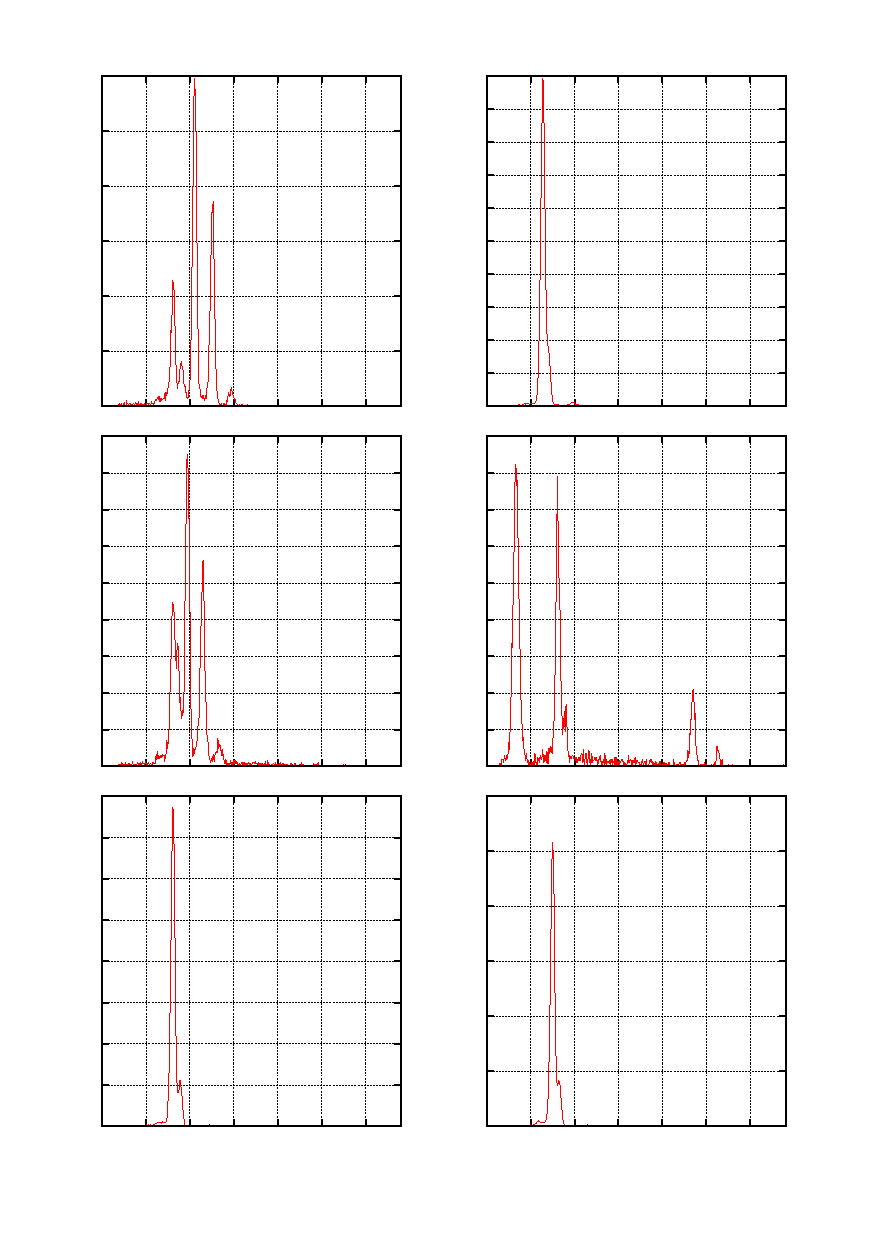
\includegraphics{./plots/referenzspektren1}}%
    \gplfronttext
  \end{picture}%
\endgroup

\end{figure}

\begin{figure}
\centering
% GNUPLOT: LaTeX picture with Postscript
\begingroup
  \makeatletter
  \providecommand\color[2][]{%
    \GenericError{(gnuplot) \space\space\space\@spaces}{%
      Package color not loaded in conjunction with
      terminal option `colourtext'%
    }{See the gnuplot documentation for explanation.%
    }{Either use 'blacktext' in gnuplot or load the package
      color.sty in LaTeX.}%
    \renewcommand\color[2][]{}%
  }%
  \providecommand\includegraphics[2][]{%
    \GenericError{(gnuplot) \space\space\space\@spaces}{%
      Package graphicx or graphics not loaded%
    }{See the gnuplot documentation for explanation.%
    }{The gnuplot epslatex terminal needs graphicx.sty or graphics.sty.}%
    \renewcommand\includegraphics[2][]{}%
  }%
  \providecommand\rotatebox[2]{#2}%
  \@ifundefined{ifGPcolor}{%
    \newif\ifGPcolor
    \GPcolortrue
  }{}%
  \@ifundefined{ifGPblacktext}{%
    \newif\ifGPblacktext
    \GPblacktexttrue
  }{}%
  % define a \g@addto@macro without @ in the name:
  \let\gplgaddtomacro\g@addto@macro
  % define empty templates for all commands taking text:
  \gdef\gplbacktext{}%
  \gdef\gplfronttext{}%
  \makeatother
  \ifGPblacktext
    % no textcolor at all
    \def\colorrgb#1{}%
    \def\colorgray#1{}%
  \else
    % gray or color?
    \ifGPcolor
      \def\colorrgb#1{\color[rgb]{#1}}%
      \def\colorgray#1{\color[gray]{#1}}%
      \expandafter\def\csname LTw\endcsname{\color{white}}%
      \expandafter\def\csname LTb\endcsname{\color{black}}%
      \expandafter\def\csname LTa\endcsname{\color{black}}%
      \expandafter\def\csname LT0\endcsname{\color[rgb]{1,0,0}}%
      \expandafter\def\csname LT1\endcsname{\color[rgb]{0,1,0}}%
      \expandafter\def\csname LT2\endcsname{\color[rgb]{0,0,1}}%
      \expandafter\def\csname LT3\endcsname{\color[rgb]{1,0,1}}%
      \expandafter\def\csname LT4\endcsname{\color[rgb]{0,1,1}}%
      \expandafter\def\csname LT5\endcsname{\color[rgb]{1,1,0}}%
      \expandafter\def\csname LT6\endcsname{\color[rgb]{0,0,0}}%
      \expandafter\def\csname LT7\endcsname{\color[rgb]{1,0.3,0}}%
      \expandafter\def\csname LT8\endcsname{\color[rgb]{0.5,0.5,0.5}}%
    \else
      % gray
      \def\colorrgb#1{\color{black}}%
      \def\colorgray#1{\color[gray]{#1}}%
      \expandafter\def\csname LTw\endcsname{\color{white}}%
      \expandafter\def\csname LTb\endcsname{\color{black}}%
      \expandafter\def\csname LTa\endcsname{\color{black}}%
      \expandafter\def\csname LT0\endcsname{\color{black}}%
      \expandafter\def\csname LT1\endcsname{\color{black}}%
      \expandafter\def\csname LT2\endcsname{\color{black}}%
      \expandafter\def\csname LT3\endcsname{\color{black}}%
      \expandafter\def\csname LT4\endcsname{\color{black}}%
      \expandafter\def\csname LT5\endcsname{\color{black}}%
      \expandafter\def\csname LT6\endcsname{\color{black}}%
      \expandafter\def\csname LT7\endcsname{\color{black}}%
      \expandafter\def\csname LT8\endcsname{\color{black}}%
    \fi
  \fi
  \setlength{\unitlength}{0.0500bp}%
  \begin{picture}(8206.00,11520.00)%
      \csname LTb\endcsname%
      \put(4103,11300){\makebox(0,0){\strut{}Referenzspektren Teil 2}}%
    \gplgaddtomacro\gplbacktext{%
      \csname LTb\endcsname%
      \put(688,7776){\makebox(0,0)[r]{\strut{}0}}%
      \csname LTb\endcsname%
      \put(688,8409){\makebox(0,0)[r]{\strut{}20}}%
      \csname LTb\endcsname%
      \put(688,9043){\makebox(0,0)[r]{\strut{}40}}%
      \csname LTb\endcsname%
      \put(688,9676){\makebox(0,0)[r]{\strut{}60}}%
      \csname LTb\endcsname%
      \put(688,10310){\makebox(0,0)[r]{\strut{}80}}%
      \csname LTb\endcsname%
      \put(688,10943){\makebox(0,0)[r]{\strut{}100}}%
      \csname LTb\endcsname%
      \put(820,7556){\makebox(0,0){\strut{} 0}}%
      \csname LTb\endcsname%
      \put(1539,7556){\makebox(0,0){\strut{} 128}}%
      \csname LTb\endcsname%
      \put(2259,7556){\makebox(0,0){\strut{} 256}}%
      \csname LTb\endcsname%
      \put(2978,7556){\makebox(0,0){\strut{} 384}}%
      \put(50,9359){\rotatebox{-270}{\makebox(0,0){\strut{}Counts}}}%
      \put(3347,10690){\makebox(0,0)[l]{\strut{}Ag}}%
    }%
    \gplgaddtomacro\gplfronttext{%
    }%
    \gplgaddtomacro\gplbacktext{%
      \csname LTb\endcsname%
      \put(4381,7776){\makebox(0,0)[r]{\strut{}0}}%
      \csname LTb\endcsname%
      \put(4381,8172){\makebox(0,0)[r]{\strut{}500}}%
      \csname LTb\endcsname%
      \put(4381,8568){\makebox(0,0)[r]{\strut{}1000}}%
      \csname LTb\endcsname%
      \put(4381,8964){\makebox(0,0)[r]{\strut{}1500}}%
      \csname LTb\endcsname%
      \put(4381,9359){\makebox(0,0)[r]{\strut{}2000}}%
      \csname LTb\endcsname%
      \put(4381,9755){\makebox(0,0)[r]{\strut{}2500}}%
      \csname LTb\endcsname%
      \put(4381,10151){\makebox(0,0)[r]{\strut{}3000}}%
      \csname LTb\endcsname%
      \put(4381,10547){\makebox(0,0)[r]{\strut{}3500}}%
      \csname LTb\endcsname%
      \put(4381,10943){\makebox(0,0)[r]{\strut{}4000}}%
      \csname LTb\endcsname%
      \put(4513,7556){\makebox(0,0){\strut{} 0}}%
      \csname LTb\endcsname%
      \put(5232,7556){\makebox(0,0){\strut{} 128}}%
      \csname LTb\endcsname%
      \put(5951,7556){\makebox(0,0){\strut{} 256}}%
      \csname LTb\endcsname%
      \put(6670,7556){\makebox(0,0){\strut{} 384}}%
      \put(7039,10690){\makebox(0,0)[l]{\strut{}Ti}}%
    }%
    \gplgaddtomacro\gplfronttext{%
    }%
    \gplgaddtomacro\gplbacktext{%
      \csname LTb\endcsname%
      \put(688,4320){\makebox(0,0)[r]{\strut{}0}}%
      \csname LTb\endcsname%
      \put(688,4716){\makebox(0,0)[r]{\strut{}100}}%
      \csname LTb\endcsname%
      \put(688,5112){\makebox(0,0)[r]{\strut{}200}}%
      \csname LTb\endcsname%
      \put(688,5508){\makebox(0,0)[r]{\strut{}300}}%
      \csname LTb\endcsname%
      \put(688,5904){\makebox(0,0)[r]{\strut{}400}}%
      \csname LTb\endcsname%
      \put(688,6299){\makebox(0,0)[r]{\strut{}500}}%
      \csname LTb\endcsname%
      \put(688,6695){\makebox(0,0)[r]{\strut{}600}}%
      \csname LTb\endcsname%
      \put(688,7091){\makebox(0,0)[r]{\strut{}700}}%
      \csname LTb\endcsname%
      \put(688,7487){\makebox(0,0)[r]{\strut{}800}}%
      \csname LTb\endcsname%
      \put(820,4100){\makebox(0,0){\strut{} 0}}%
      \csname LTb\endcsname%
      \put(1539,4100){\makebox(0,0){\strut{} 128}}%
      \csname LTb\endcsname%
      \put(2259,4100){\makebox(0,0){\strut{} 256}}%
      \csname LTb\endcsname%
      \put(2978,4100){\makebox(0,0){\strut{} 384}}%
      \put(50,5903){\rotatebox{-270}{\makebox(0,0){\strut{}Counts}}}%
      \put(3347,7234){\makebox(0,0)[l]{\strut{}W}}%
    }%
    \gplgaddtomacro\gplfronttext{%
    }%
    \gplgaddtomacro\gplbacktext{%
      \csname LTb\endcsname%
      \put(4381,4320){\makebox(0,0)[r]{\strut{}0}}%
      \csname LTb\endcsname%
      \put(4381,4953){\makebox(0,0)[r]{\strut{}50}}%
      \csname LTb\endcsname%
      \put(4381,5587){\makebox(0,0)[r]{\strut{}100}}%
      \csname LTb\endcsname%
      \put(4381,6220){\makebox(0,0)[r]{\strut{}150}}%
      \csname LTb\endcsname%
      \put(4381,6854){\makebox(0,0)[r]{\strut{}200}}%
      \csname LTb\endcsname%
      \put(4381,7487){\makebox(0,0)[r]{\strut{}250}}%
      \csname LTb\endcsname%
      \put(4513,4100){\makebox(0,0){\strut{} 0}}%
      \csname LTb\endcsname%
      \put(5232,4100){\makebox(0,0){\strut{} 128}}%
      \csname LTb\endcsname%
      \put(5951,4100){\makebox(0,0){\strut{} 256}}%
      \csname LTb\endcsname%
      \put(6670,4100){\makebox(0,0){\strut{} 384}}%
      \put(7039,7234){\makebox(0,0)[l]{\strut{}Sn}}%
    }%
    \gplgaddtomacro\gplfronttext{%
    }%
    \gplgaddtomacro\gplbacktext{%
      \csname LTb\endcsname%
      \put(688,863){\makebox(0,0)[r]{\strut{}0}}%
      \csname LTb\endcsname%
      \put(688,1259){\makebox(0,0)[r]{\strut{}500}}%
      \csname LTb\endcsname%
      \put(688,1655){\makebox(0,0)[r]{\strut{}1000}}%
      \csname LTb\endcsname%
      \put(688,2051){\makebox(0,0)[r]{\strut{}1500}}%
      \csname LTb\endcsname%
      \put(688,2447){\makebox(0,0)[r]{\strut{}2000}}%
      \csname LTb\endcsname%
      \put(688,2843){\makebox(0,0)[r]{\strut{}2500}}%
      \csname LTb\endcsname%
      \put(688,3239){\makebox(0,0)[r]{\strut{}3000}}%
      \csname LTb\endcsname%
      \put(688,3635){\makebox(0,0)[r]{\strut{}3500}}%
      \csname LTb\endcsname%
      \put(688,4031){\makebox(0,0)[r]{\strut{}4000}}%
      \csname LTb\endcsname%
      \put(820,643){\makebox(0,0){\strut{} 0}}%
      \csname LTb\endcsname%
      \put(1539,643){\makebox(0,0){\strut{} 128}}%
      \csname LTb\endcsname%
      \put(2259,643){\makebox(0,0){\strut{} 256}}%
      \csname LTb\endcsname%
      \put(2978,643){\makebox(0,0){\strut{} 384}}%
      \put(-82,2447){\rotatebox{-270}{\makebox(0,0){\strut{}Counts}}}%
      \put(2256,313){\makebox(0,0){\strut{}Kanalnummer}}%
      \put(3347,3778){\makebox(0,0)[l]{\strut{}Zn}}%
    }%
    \gplgaddtomacro\gplfronttext{%
    }%
    \gplgaddtomacro\gplbacktext{%
      \csname LTb\endcsname%
      \put(4381,863){\makebox(0,0)[r]{\strut{}0}}%
      \csname LTb\endcsname%
      \put(4381,1259){\makebox(0,0)[r]{\strut{}100}}%
      \csname LTb\endcsname%
      \put(4381,1655){\makebox(0,0)[r]{\strut{}200}}%
      \csname LTb\endcsname%
      \put(4381,2051){\makebox(0,0)[r]{\strut{}300}}%
      \csname LTb\endcsname%
      \put(4381,2447){\makebox(0,0)[r]{\strut{}400}}%
      \csname LTb\endcsname%
      \put(4381,2843){\makebox(0,0)[r]{\strut{}500}}%
      \csname LTb\endcsname%
      \put(4381,3239){\makebox(0,0)[r]{\strut{}600}}%
      \csname LTb\endcsname%
      \put(4381,3635){\makebox(0,0)[r]{\strut{}700}}%
      \csname LTb\endcsname%
      \put(4381,4031){\makebox(0,0)[r]{\strut{}800}}%
      \csname LTb\endcsname%
      \put(4513,643){\makebox(0,0){\strut{} 0}}%
      \csname LTb\endcsname%
      \put(5232,643){\makebox(0,0){\strut{} 128}}%
      \csname LTb\endcsname%
      \put(5951,643){\makebox(0,0){\strut{} 256}}%
      \csname LTb\endcsname%
      \put(6670,643){\makebox(0,0){\strut{} 384}}%
      \put(5948,313){\makebox(0,0){\strut{}Kanalnummer}}%
      \put(7039,3778){\makebox(0,0)[l]{\strut{}Zr}}%
    }%
    \gplgaddtomacro\gplfronttext{%
    }%
    \gplbacktext
    \put(0,0){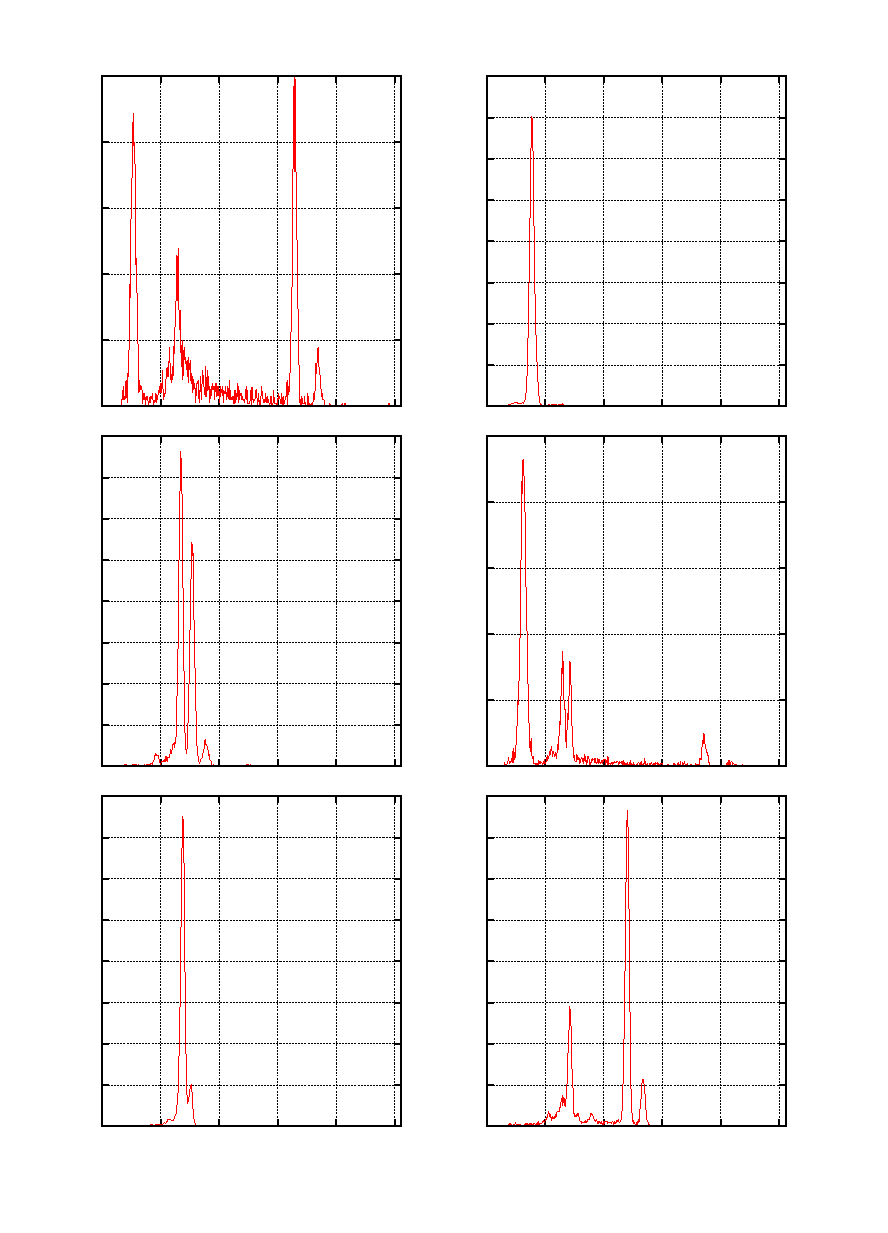
\includegraphics{./plots/referenzspektren2}}%
    \gplfronttext
  \end{picture}%
\endgroup

\end{figure}

% BIBLIOGRAPHIE

% Maximale Anzahl der Einträge in Klammer
% Zitieren mit \cite{lamport94}
\begin{thebibliography}{9}

% Beispiel
\bibitem{lamport94}
  Leslie Lamport,
  \emph{\LaTeX: a document preparation system}.
  Addison Wesley, Massachusetts,
  2nd edition,
  1994.

\bibitem{demtroeder}
	Wolfgang Demtröder,
	\emph{Experimentalphysik 3}.
	Springer Verlag,
	3. Auflage
\end{thebibliography}


\newpage

% APPENDIX
\begin{appendix}

\end{appendix}

\end{document}
